\documentclass[12pt,a4paper]{article}
\usepackage[top=2.7cm, bottom=2cm, left=2cm, right=2cm]{geometry}
\usepackage[utf8]{inputenc}
\usepackage{CJKutf8}
\usepackage{enumitem}
\usepackage{verbatim}


%% Useful packages
\usepackage{amsmath,amssymb}
% \usepackage{subfigure}
\usepackage{graphicx,wrapfig}
\usepackage[dvipsnames,table]{xcolor}
\usepackage[table]{xcolor}
\usepackage{url}
\usepackage{setspace}
\usepackage[colorlinks=true,anchorcolor=black,linkcolor=Blue,urlcolor=RoyalBlue]{hyperref}
\usepackage[linesnumbered,ruled,vlined]{algorithm2e}
\usepackage{threeparttable}

\usepackage{tikz}
\usepackage{blindtext}
\usepackage{titlesec}
\usepackage{courier}
\usepackage{pdfpages}

\usepackage{lastpage}
\usepackage{fancyhdr}
\setlength{\headheight}{0pt}
\renewcommand{\headrulewidth}{1pt} % remove lines
\renewcommand{\footrulewidth}{0pt}
\pagestyle{fancyplain}
\fancyhf{}
\lhead{
  \textcolor{Gray}{Group 2}
}
\rhead{
  \begin{CJK}{UTF8}{bkai}
  \textcolor{Gray}{實驗物理學結報}
  \end{CJK}
}
\lfoot{
   \textcolor{Gray}{Feburary 25}
  }
\rfoot{
  \thepage/\pageref{LastPage}
  }

\title{\vspace{-0.5cm}
       {\bf \textcolor{black}{{\LARGE 
       \begin{CJK}{UTF8}{bkai}
       實驗物理學(二)\\
       \vspace{6pt}
       實驗結報\\
       \vspace{60pt}
       實驗一、複習基本儀器使用與原理
       \end{CJK}
       }}
       }
       }
\author{}
\date{}

\begin{document}
\begin{CJK}{UTF8}{bkai}

\maketitle
\thispagestyle{empty}

\vspace{10cm}
\begin{center}
{\large 第二組}\\ \vspace{12pt}
{\large \makebox[3em][s]{洪\hspace{\fill}瑜} B125090009}\\ \vspace{6pt}
{\large \makebox[3em][s]{黃巧涵}  B122030003}\\ \vspace{6pt}
{\large \makebox[3em][s]{洪懌平} B102030019}\\ \vspace{12pt}
{\large 2025/02/25}\\
\end{center}

\clearpage

\section{實驗目的}

\begin{enumerate}
    \item 確認麵包板的運作原理(實驗一;Sec.\ref{subsec:step_1})
    \item 熟悉以電腦軟體PicoScope操控示波器和相關電子設備的操作(實驗二;Sec.\ref{subsec:step_2})
    \item 透過訊號產生器改變不同頻率,以得知頻率和直流電訊號之關係(實驗三;Sec.\ref{subsec:step_3})
    \item 透過量測不同歐姆檔位的電壓,推測三用電表的內電阻(實驗四;Sec.\ref{subsec:step_4})
    \item 透過串連電阻將電壓分壓(實驗五;Sec.\ref{subsec:step_5})
\end{enumerate}

\section{實驗原理}
\subsection{麵包板測量原理}
\hfill

可透過歐姆定律得知孔位的連接性
\begin{itemize}
    \item 若兩孔位相通,$R \sim$ 0
    \item 若兩孔位不通,$R \sim\infty$
\end{itemize}

\subsection{訊號產生器和正弦波}\label{subsec:princ_2}
\hfill

訊號產生器可產生不同頻率、振幅的正弦訊號,用下述公式表示:
\begin{equation}
V(t)=V_{pp}sin(2\pi ft+\phi)+V_{DC}
\end{equation}
其中$V_{pp}$為峰對峰值、$f$為頻率、$t$為時間、$\phi$為相位、$V_{DC}$為直流偏移(DC offset)

\subsection{電表測量AC和DC之方式}
\hfill

\begin{itemize}
    \item DCV(直流電壓檔):\\
    測量訊號的直流電壓(DC offset),其通常通過低通濾波器將交流訊號過濾。
    \item ACV(交流電壓檔):\\
    電表會測量其訊號交流成分,但不包含直流偏移(DC Offset),而其測量使用均方根(RMS, Root Mean Square )電壓:
    \begin{equation}
        V_{RMS}=\frac{V_{pp}}{\sqrt{2}}
    \end{equation}
\end{itemize}


若此時訊號為DC+AC,例如:
\begin{equation}
    V(t) = 1+sin(2\pi ft)
\end{equation}
而電表的DCV檔只測量直流部分(1V),不會顯示交流部分(1V sine wave),濾波器已經去除大部分AC成分。

這也是在實驗中:
\begin{itemize}
    \item $V_{DC}$= 0V,DCV讀數為0V(因為訊號的平均為0)
    \item $V_{DC}$=+1V,DCV讀數為1V (因為訊號的平均為1V)
\end{itemize}

\subsection{分壓器}
\hfill

一個由兩個串聯電阻組成的電路,根據歐姆定律,分壓器之輸出電壓$V_{out}$可用下列公式計算:
\begin{equation}
\label{eq:r1r2}
    V_{out} = V_{in}\frac{R_{2}}{R_{1}+R_{2}}
\end{equation}
其中$V_{in}$為輸入電壓、$R_{1}$和$R_{2}$為串聯之電阻、$V_{out}$為輸出電壓


\section{實驗步驟}
\subsection{實驗一:麵包板}\label{subsec:step_1}
\begin{enumerate}
    \item 規劃不同線路的連接方式
    \item 按照所規劃之連接方式實際操作於麵包板
    \item 確認實際操作之結果與理論相符
\end{enumerate}

\subsection{實驗二:複習示波器和訊號產生器}\label{subsec:step_2}

\begin{enumerate}
    \item 利用機器所附連接線將PicoScope連接於筆電(Fig.\ref{fig:step}左)
    \item 本實驗利用Channel A量測,故將線路接至Channel A(最左側)之連接口,並與訊號產收器進行連接
    \item 確認設備運作正常
    \item 透過調整訊號產生器輸出之弦波訊號頻率及DC offset,得出個弦波訊號之圖樣
\end{enumerate}

\subsection{實驗三:電表的電壓檔}\label{subsec:step_3}

\begin{enumerate}
    \item 透過示波器調整訊號產生器到指定參數($f$=100 Hz; $V_{pp}$ = 2V; $V_{DC}$=0)
    \item 使用三用電表的DCV檔位及ACV檔位量測電壓值
    \item 調整$V_{DC}$=+1V,重複步驟2.
    \item 調整訊號產生器頻率至100KHz、1MHz,並測量其在$V_{DC}$ =0 和$V_{DC}$=+1V時的DCV和ACV數值。
\end{enumerate}

\subsection{實驗四:歐姆檔}\label{subsec:step_4}

\begin{enumerate}
    \item 將三用電表A調整至電壓檔位、並將三用電表B調整至電阻檔位,連接三用電表A及三用電表B (見Fig. \ref{fig:step}中)
    \item 連接後,接三用電表B切換不同的電阻檔位,並記錄其電壓值
    \item 將上述裝置串連一個電阻(使用10$\Omega$和1k$\Omega$)重複步驟2.
\end{enumerate}

\subsection{實驗五:分壓器}\label{subsec:step_5}

\begin{enumerate}
    \item 連接電路如Fig.\ref{fig:step}右
    \item $V_{in}$=5V(由電源供應器提供),電阻分別使用10k、100k、1M和10M$\Omega$
    \item 使用三用電表測量$V_{out}$
    \item 使用PicoScope軟體調整訊號產生器的參數($f$=100 Hz; $V_{pp}$ = 10V; $V_{DC}$=0)
    \item 將電路和示波器連結,並使用其探針($\times$1)測量 $V_{out}$
    \item 切換探針至($\times$10),並重複上述步驟
\end{enumerate}

% \begin{figure}[h]
%     \centering
%     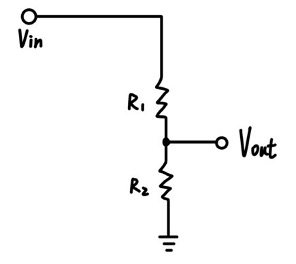
\includegraphics[width=0.25\linewidth]{figures/exp_5.jpg}
%     \caption{實驗五線路示意圖}
%     \label{fig:exp_5}
% \end{figure}

\begin{figure}[h]
    \centering
    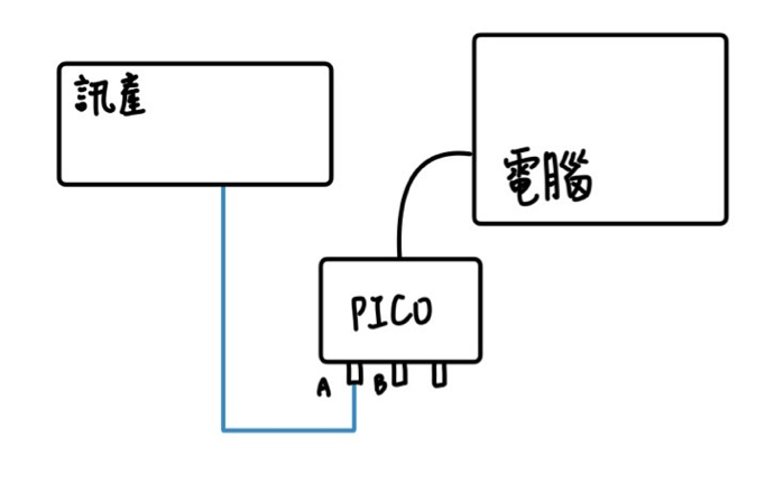
\includegraphics[width=0.45\linewidth]{figures/exp_2.png}
    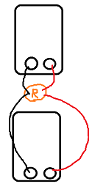
\includegraphics[width=0.15\linewidth]{figures/exp_4.png}
    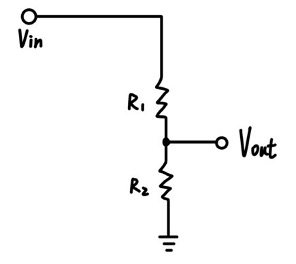
\includegraphics[width=0.3\linewidth]{figures/exp_5.jpg}
    \caption{實驗線路示意圖(左:實驗二;中:實驗四;右:實驗五)}
    \label{fig:step}
\end{figure}

\clearpage

\section{實驗結果和分析}

\subsection{實驗一:麵包板}

\begin{figure}[h]
    \centering
    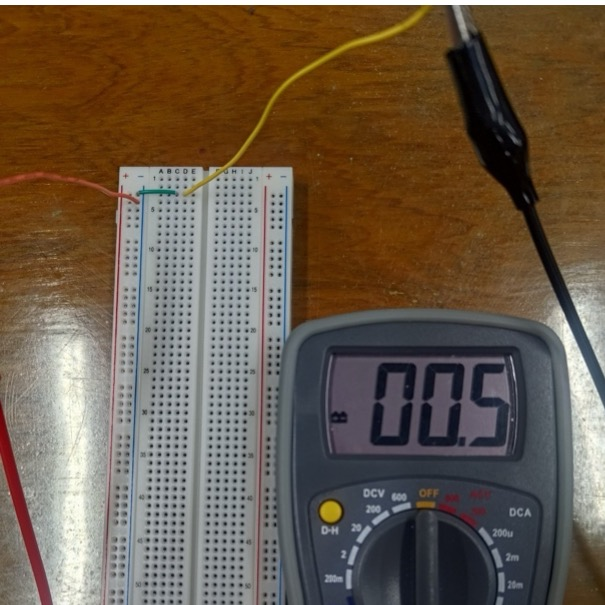
\includegraphics[width=0.45\linewidth]{figures/exp1/exp1_1.jpg}
    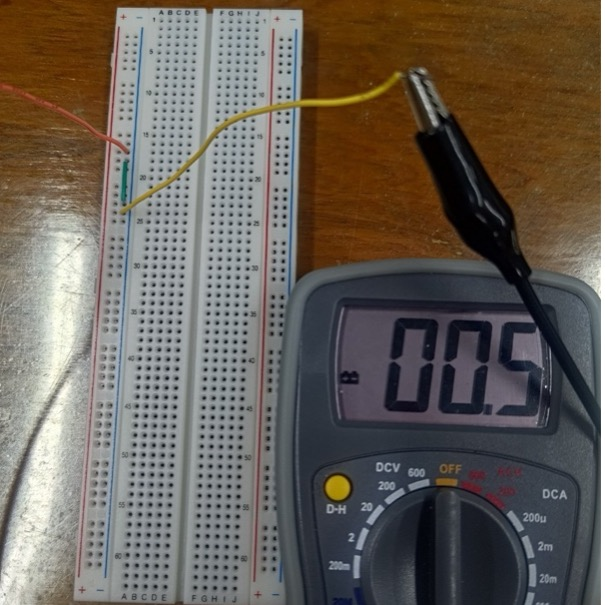
\includegraphics[width=0.45\linewidth]{figures/exp1/exp1_2.jpg}\\
    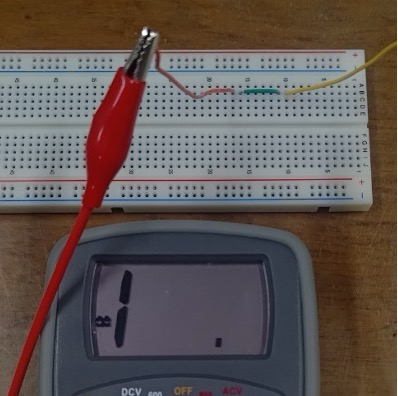
\includegraphics[width=0.45\linewidth]{figures/exp1/exp1_3.jpg}
    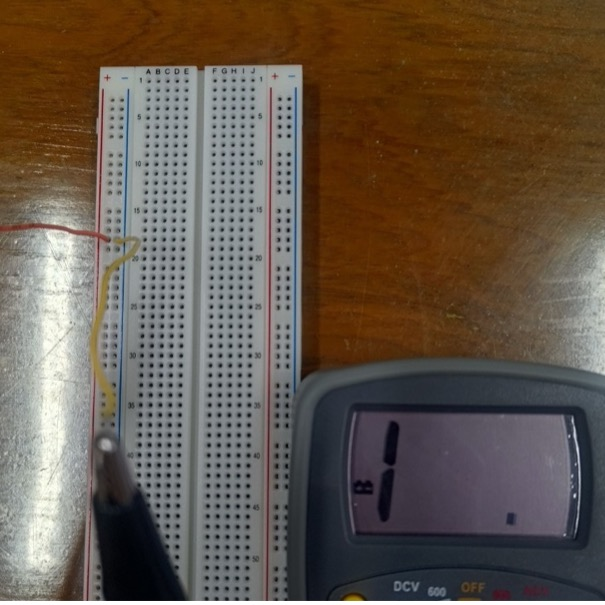
\includegraphics[width=0.45\linewidth]{figures/exp1/exp1_4.jpg}
    \caption{麵包板不同接線方式之接通狀態(左上右上:通路;左下右下:斷路)}
    \label{fig:exp1_result}
\end{figure}

通過在麵包板上連接的情況,可以得到我們所測之各孔間的導通狀態與實驗理論相符:若將麵包板以直向擺放時,左右兩側之孔洞為縱向導通;中間的孔洞以橫向導通。\\
將三用電錶轉至歐姆檔,倘若三用電錶測量之數值趨近0時,則表電路接通;反之,螢幕因電阻過大而顯示不出數值時,則表示電路未導通。

\clearpage
\subsection{實驗二:複習示波器和訊號產生器}
\hfill
\begin{enumerate}
    \item 無任何訊號連接之情況:
    \begin{figure}[h]
        \centering
        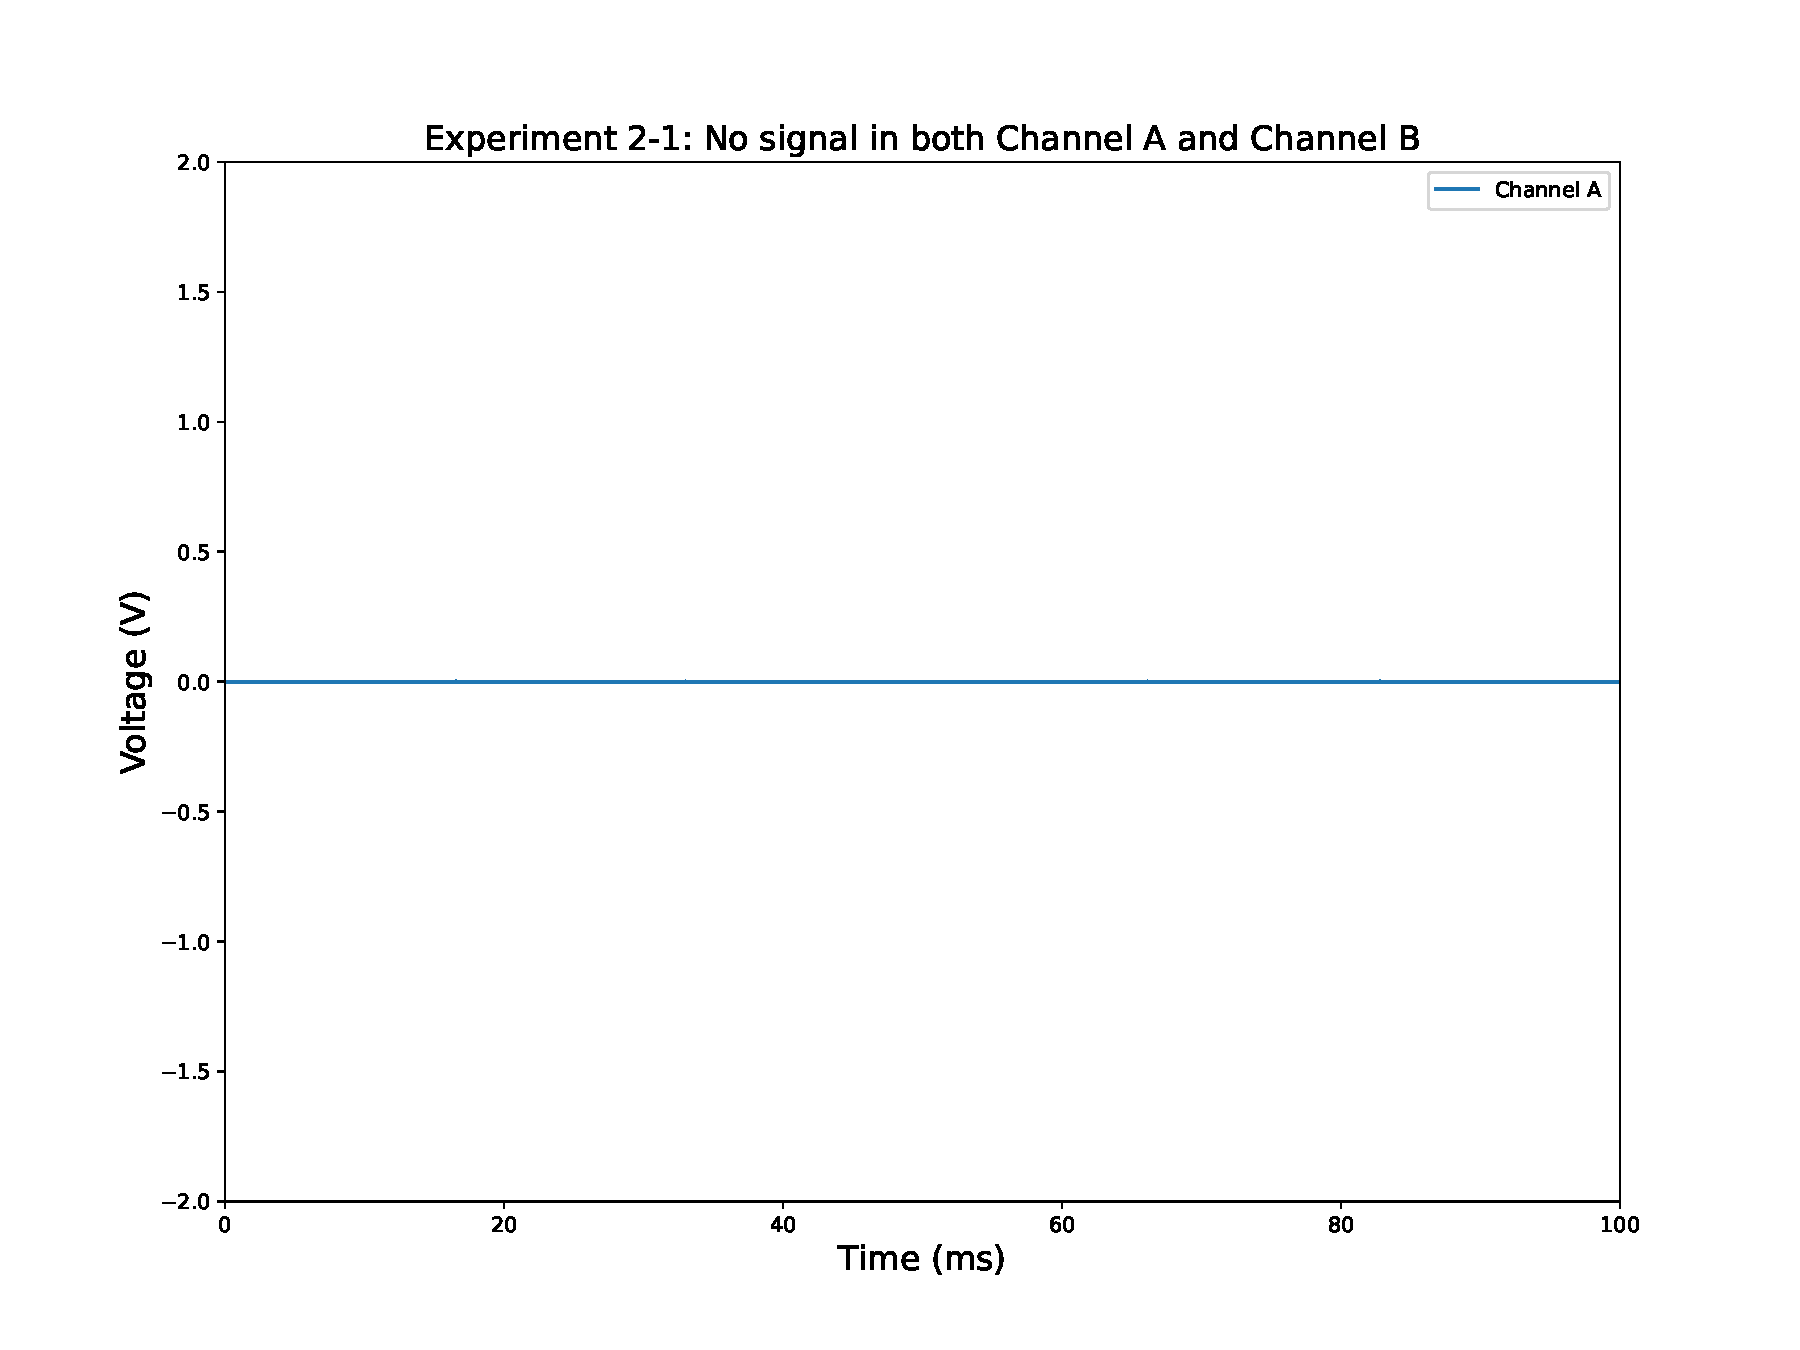
\includegraphics[width=0.85\linewidth]{figures/exp2/exp2-1.pdf}
        \caption{無任何訊號連接之情況}
        \label{fig:exp2_1}
    \end{figure}
    
    % \hfill
    由於沒有連接訊號,示波器所偵測並顯示出的圖形應為一條水平直線。但從圖表中可看見仍有少許起伏。推測是因為此示波器的靈敏度較高,並受到其他雜訊影響,如環境干擾(桌面震動、其他電子設備)或是示波器內部產生之雜訊。若想要進一步減少雜訊影響,可考慮減少示波器頻寬,或增加示波器的電壓範圍。此實驗使用的是PicoScope示波器,因此也可以透過更換供電設備,或是使用品質較好之USB線連接器材。
    
    \clearpage
    \item 調整訊號產生器至參數:$f$=200 Hz; $V_{pp}$=1V; $V_{DC}$=0V
    \begin{figure}[h]
        \centering
        \vspace{-0.8cm}
        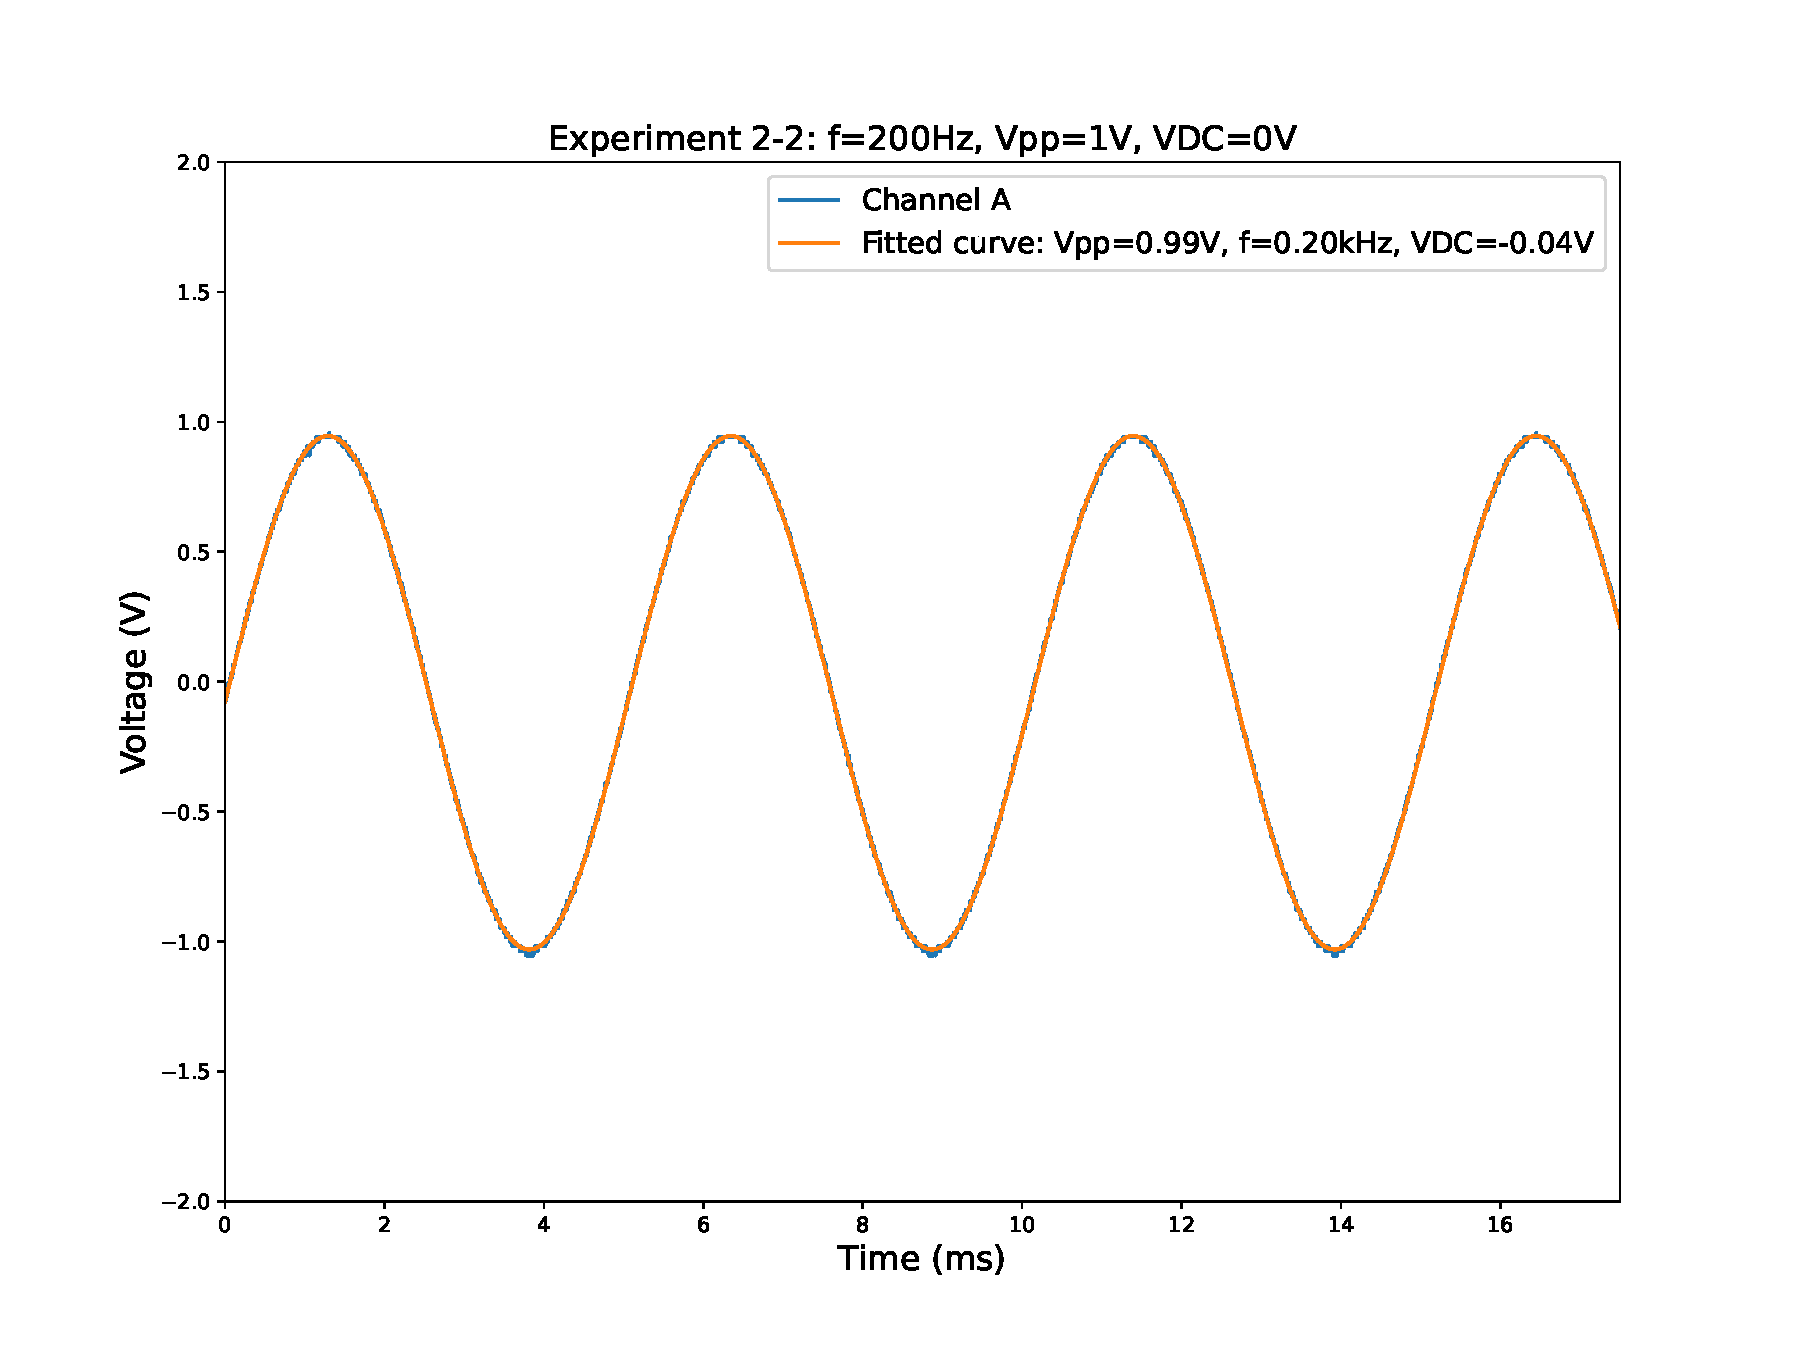
\includegraphics[width=0.75\linewidth]{figures/exp2/exp2-2.pdf}
        \vspace{-0.5cm}
        \caption{$f$=200 Hz, $V_{pp}$=1V,$V_{DC}$=0V}
        \label{fig:exp2_2}
    \end{figure}
    
    \item 調整訊號產生器至參數:$f$=200 Hz; $V_{pp}$=1V; $V_{DC}$=1V
    \begin{figure}[h]
        \centering
        \vspace{-0.8cm}
        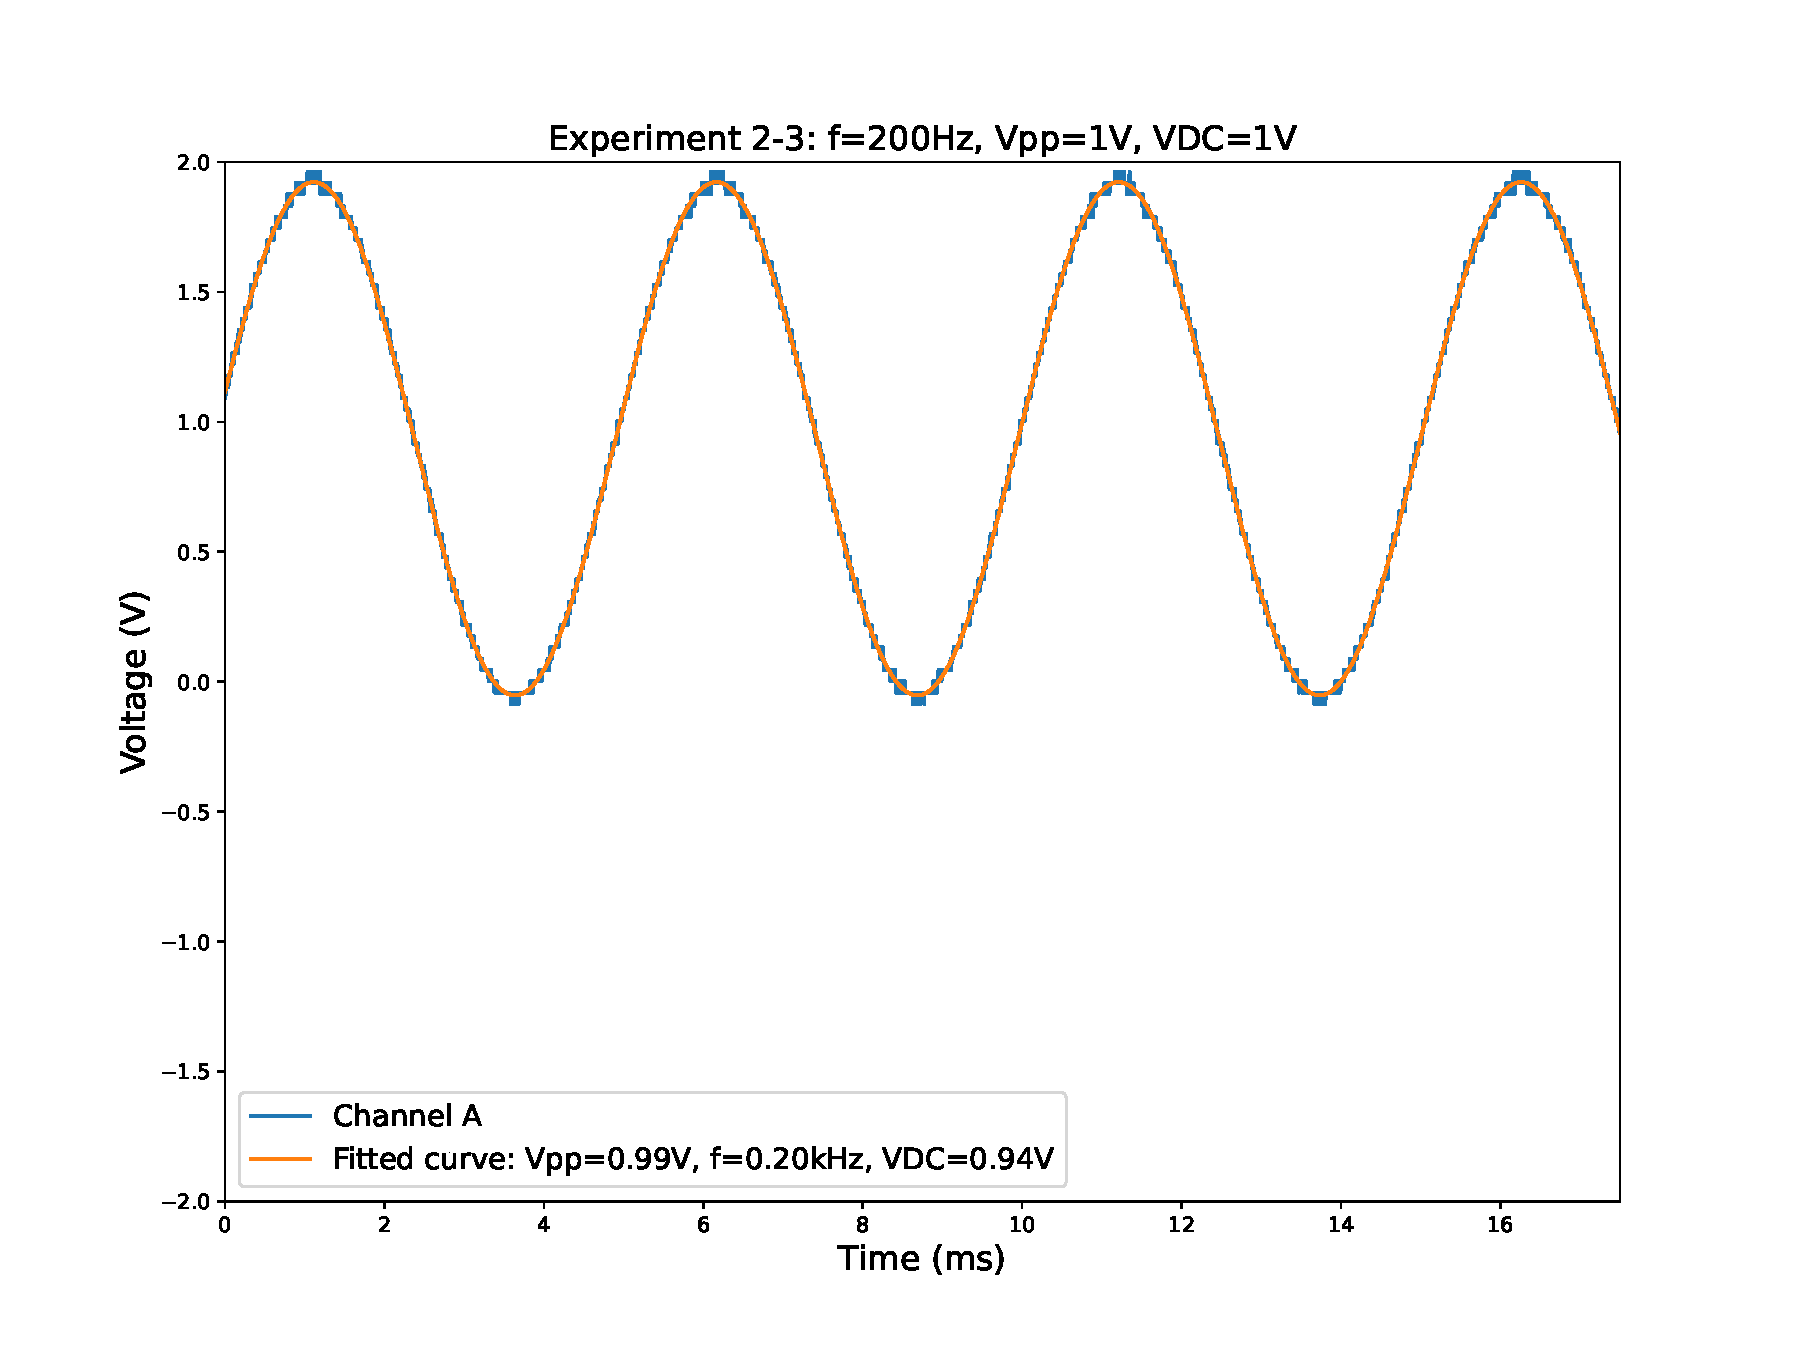
\includegraphics[width=0.75\linewidth]{figures/exp2/exp2-3.pdf}
        \vspace{-0.5cm}
        \caption{$f$=200 Hz; $V_{pp}$=1V; $V_{DC}$=1V}
        \label{fig:exp2_3}
    \end{figure}
    \clearpage
    
    \item 調整訊號產生器至參數:$f$=2 kHz; $V_{pp}$=1V; $V_{DC}$=0V
    \begin{figure}[h]
        \centering
        \vspace{-0.8cm}
        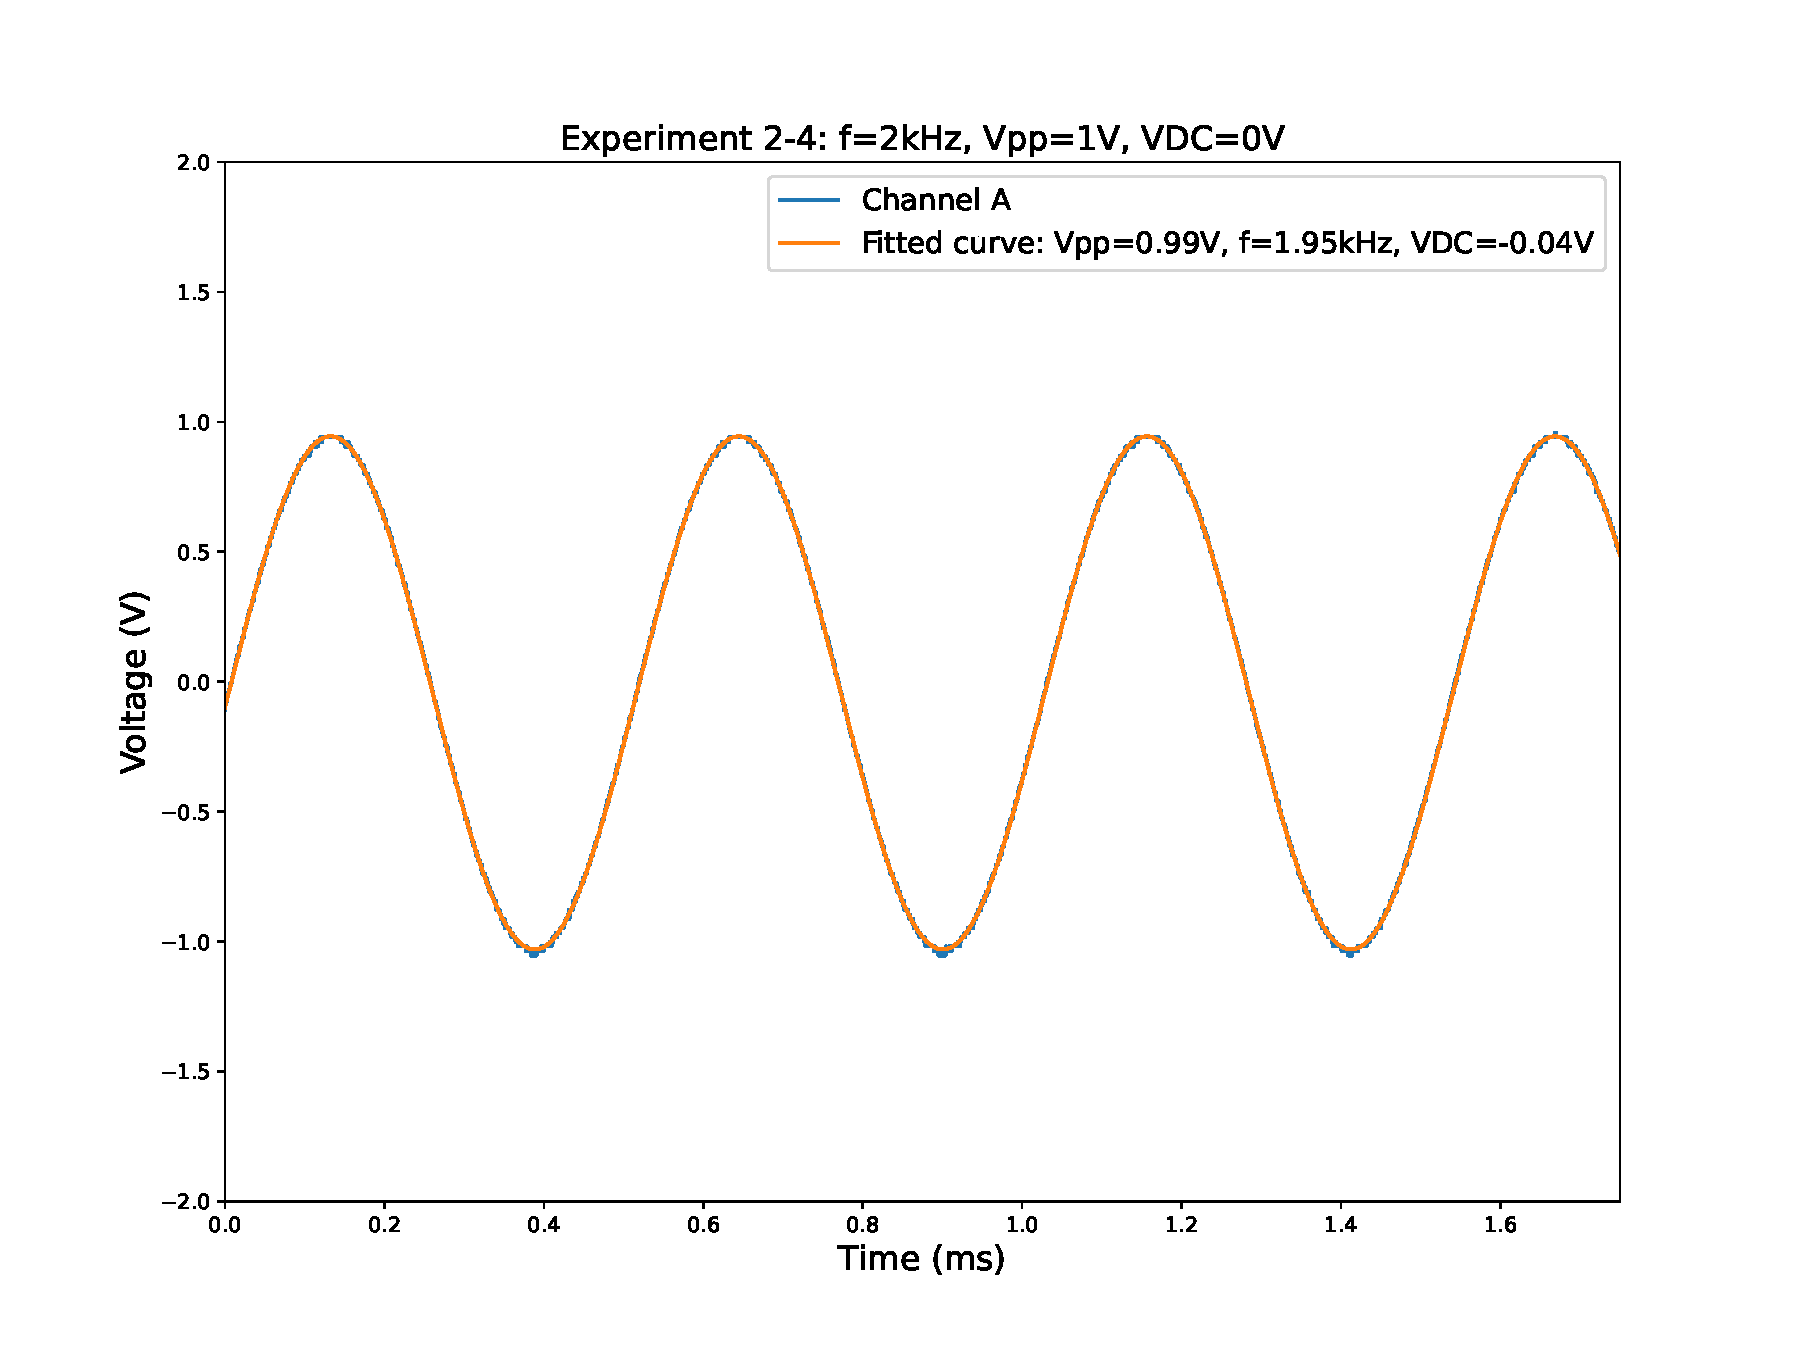
\includegraphics[width=0.75\linewidth]{figures/exp2/exp2-4.pdf}
        \vspace{-0.5cm}
        \caption{$f$=2 kHz; $V_{pp}$=1V; $V_{DC}$=0V}
        \label{fig:exp2_4}
    \end{figure}
    
    \item 調整訊號產生器至參數:$f$=2 kHz; $V_{pp}$=1V; $V_{DC}$=1V
    \begin{figure}[h]
        \centering
        \vspace{-0.8cm}
        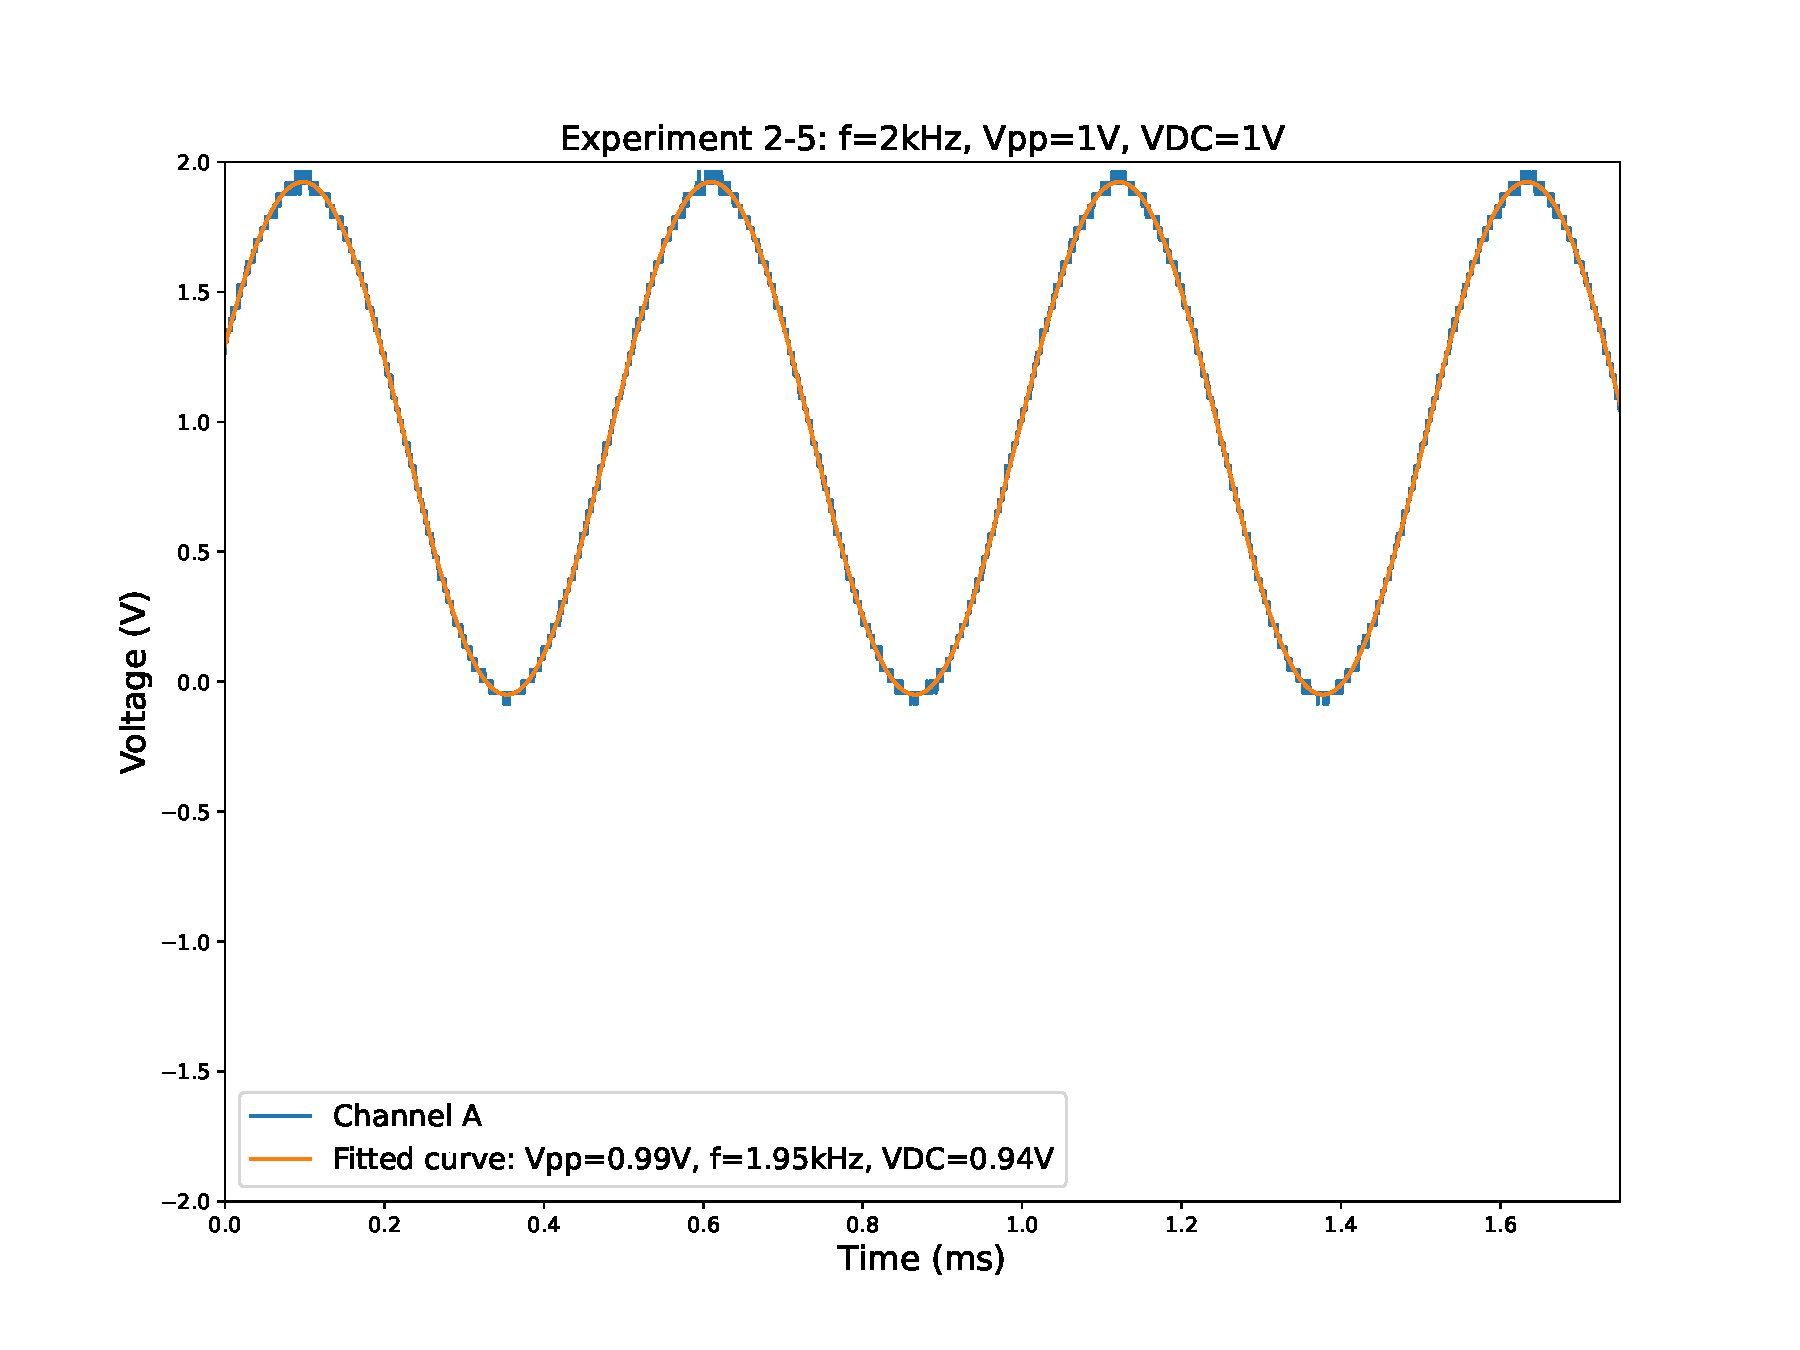
\includegraphics[width=0.75\linewidth]{figures/exp2/exp2-5.pdf}
        \vspace{-0.5cm}
        \caption{$f$=200 Hz; $V_{pp}$=1V; $V_{DC}$=1V}
        \label{fig:exp2_5}
    \end{figure}
    \clearpage
\end{enumerate}

\begin{figure}
        \centering
        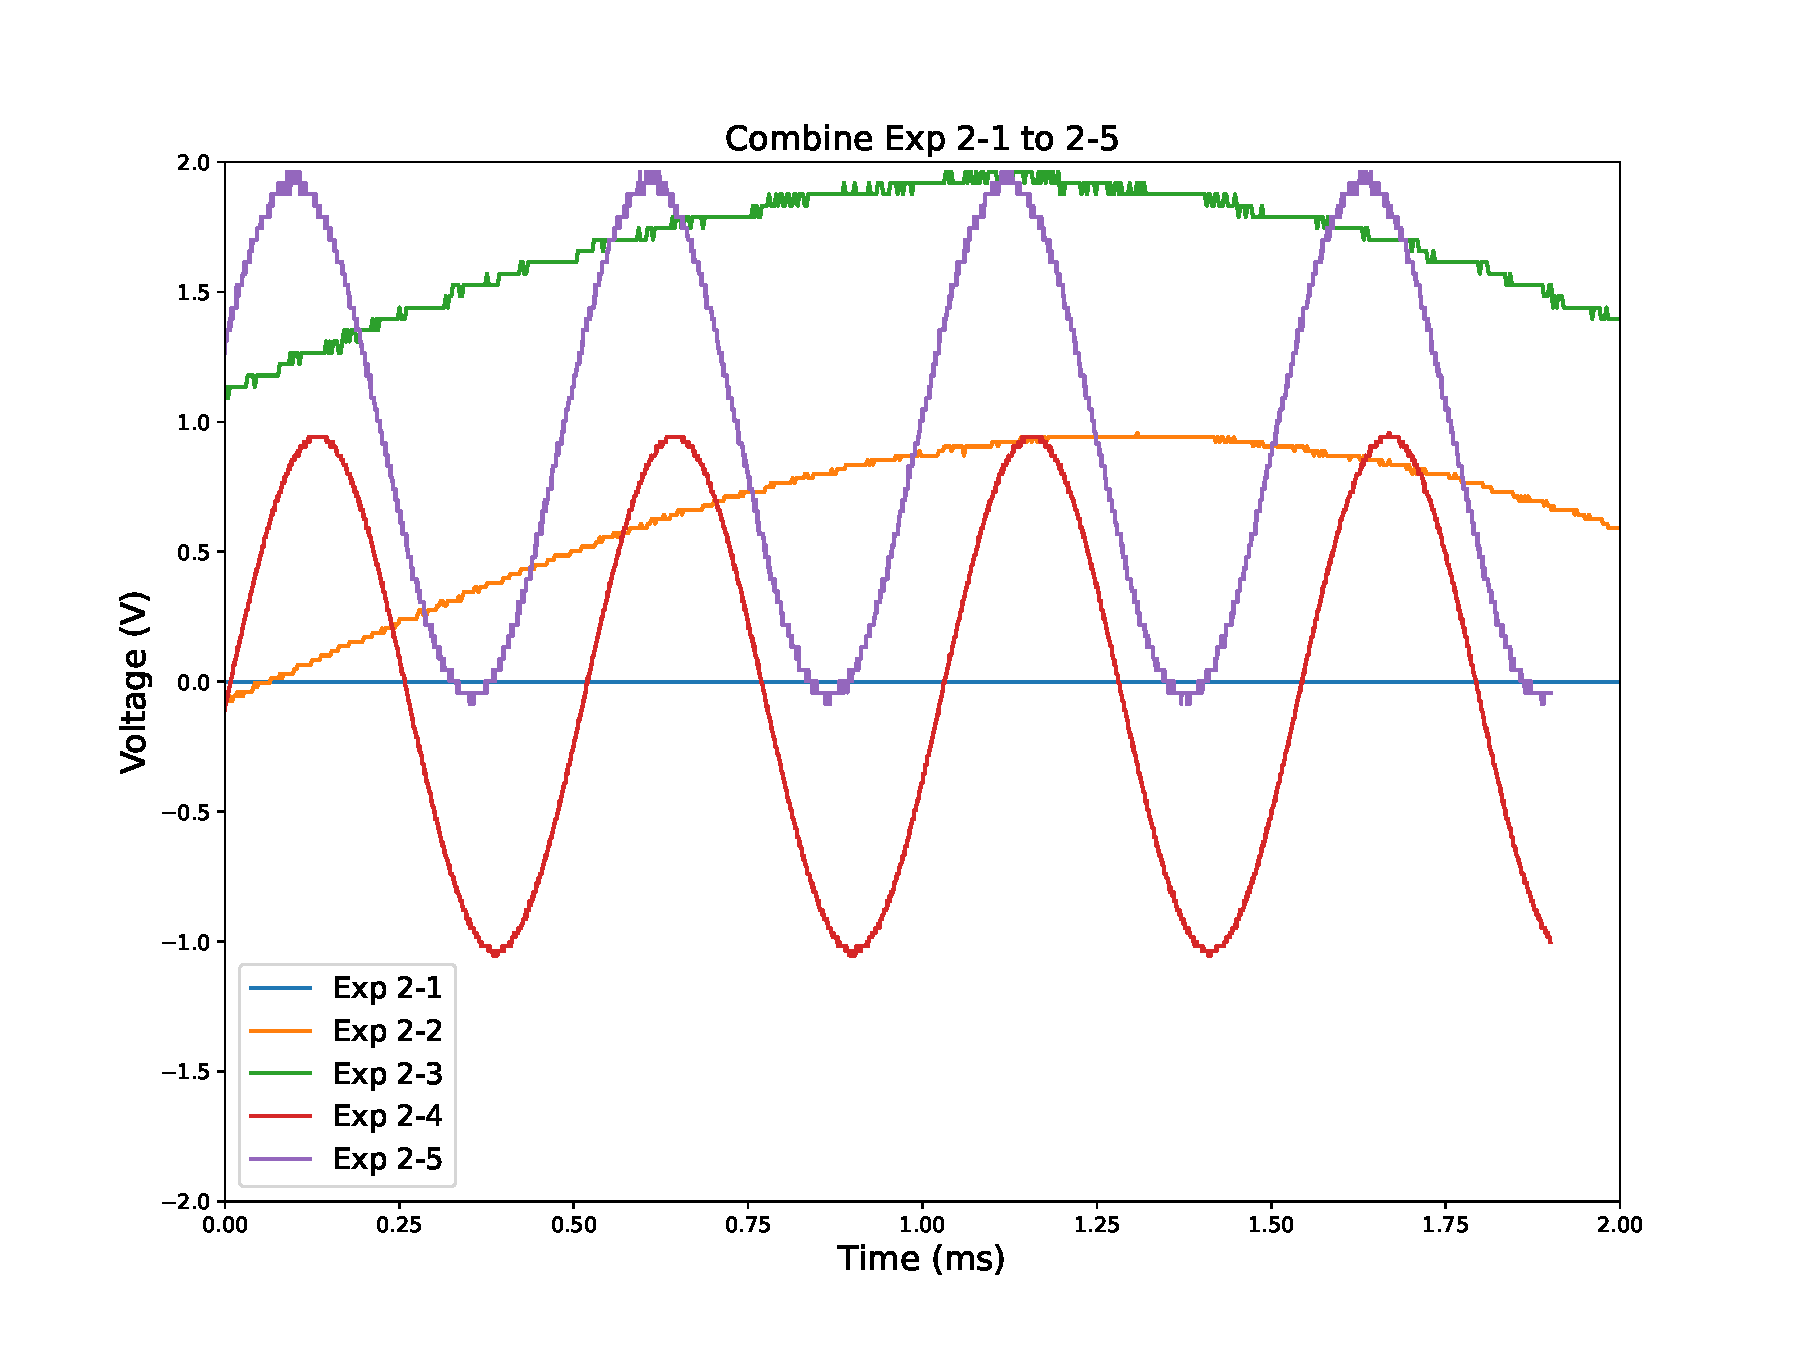
\includegraphics[width=0.8\linewidth]{figures/exp2/combine.pdf}
        \caption{實驗2-1到2-5數據}
        \label{fig:enter-label}
    \end{figure}
    
    根據實驗原理Sec.\ref{subsec:princ_2},波形須符合:
    \begin{equation}
    \label{eq: vt}
        V(t) = V_{pp}sin(2\pi ft)+V_{DC}
    \end{equation}
    藉Eq.\ref{eq: vt},可對實驗2-2到2-5之數據做擬合,可得實際數據的$V_{pp}$、$f$和$V_{DC}$。(詳細參數可見Fig. \ref{fig:exp2_2}-\ref{fig:exp2_5}圖內標示)
    由這些數據,我們可推知:
    \begin{itemize}
        \item 由於訊號產生器的旋鈕無法精準至$V_{pp}$= 1.00V,故皆使用最接近的$V_{pp}$= 0.99V進行量測
        \item 實驗2-2與2-4的 DC offset ($V_{DC}$)接皆等於 0V,因此Fig.\ref{fig:exp2_2}與Fig.\ref{fig:exp2_4}之波形皆對稱於0V,且最大值為+1V,最小值為-1V
        \item 實驗2-3與2-5的 DC offset 同樣因旋鈕精準度,只能調到最接近1V的0.94V。同樣帶入\ref{eq: vt}可得知波形應向上平移0.94V,此時訊號最大值為+1.94V,最小值則應為-0.06V。對照實際數據(Fig.\ref{fig:exp2_3}和Fig.\ref{fig:exp2_5}),確認實際測值與理論相符。
    \end{itemize}

\clearpage
\subsection{實驗三:電表的電壓檔}

\begin{center}
    \begin{tabular}{c|c|c|c|c|c|c|c}
    實驗  &   頻率  &   $V_{pp}$    &   DC offset   &   DCV read    &   DCV ideal   &   ACV read    &   ACV ideal  \\\hline
        &   (Hz)    & \multicolumn{6}{c}{(V)}\\
    \hline
    \hline
    3-1 &   100   &   2  &   0  &   0.05    &   0   &   0.04    &   0.707\\\hline
    3-2 &   100 &   2   &   1   &   1.10    &   1   &   1.80    &   0.707\\\hline
    3-3 &   100k &   2   &   0   &   $<$0.00    &   0   &   $<$0.00    &   0.707\\\hline
    3-4 &   100k &   2   &   1   &   1.10    &   1   &   1.80    &   0.707\\\hline
    \end{tabular}
\end{center}

DC offset 除了會讓訊號在波形上產生偏移,在使用某些無法正確分辨出AC與DC訊號的量測工具(如三用電表)時,會導致量測出的數據與理論數字有落差。三用電表的ACV量測內建低通濾波器,頻率約為50Hz-1kHz ,故在參數頻率為100kHz時,AC訊號已超出量測範圍 。且三用電表的 ACV 測量在接近其上限頻率時可能開始衰減,而非直接完全無法測量,故讀值顯示為$<$0.00V。

量測低頻訊號(100Hz)時, ACV 讀值應為純 AC 訊號的 RMS 值 ,但ACV檔位的量測數值可能因電表的頻率響應而產生偏差,導致ACV實際讀值小於理論值。理論上 ACV 讀值不應受 DC Offset 影響,但由於三用電表缺乏高通濾波(AC 耦合功能) ,導致DC offset也會影響ACV讀值。相較之下,DCV 只取 DC Offset,不受頻率影響,應該等於設定的 Offset 值。三用電表因為在高頻時可能會導致AC讀值衰減。若選用示波器進行量測,則可得出更精準的RMS值。

\subsection{實驗四:電表的歐姆檔}

此實驗的目的是透過不同檔位的三用電錶在歐姆檔下測量開路電壓 ($V_{out}$) 和串聯已知電阻的分壓情況,推測三用電錶的內部電壓源 ($V_{a}$) 和內部輸出阻抗 ($R_{out}$)。

\begin{enumerate}
    \item 無電阻的情況將三用電表和三用電表\\
    \begin{center}
    \begin{tabular}{c|c}
    \hline
    電阻檔$\Omega$    &   $V_{out}$(V)\\
    \hline
    \hline
    20M &   0.22\\\hline
    200k    &   0.41\\\hline
    20k &   0.41\\\hline
    2k  &   0.42\\\hline
    200 &   0.40\\\hline
    \end{tabular}
    \end{center}
    由此可見,在 200k$\Omega$、20k$\Omega$、2k$\Omega$、200$\Omega$ 檔時,開路電壓約為 0.40 ~ 0.42V,而 20M$\Omega$ 檔較低,約為 0.22V。這表示不同檔位的內部電路不同,但我們可以合理假設內部電壓源 $V_{a}$ 約為 0.4V(取 0.41V 作為近似值)。\\
    當三用電錶測量某個已知電阻  $R_x$  時,它實際上與內部輸出阻抗$R_{out}$形成分壓電路,公式為:
    \begin{equation}
    \label{eq:va_rout}
        V_{out} = V_{a} \frac{R_{x}}{R_{out}+R_{x}}
    \end{equation}
    我們可以利用這個公式來推導不同檔位下的$R_{out}$
    \clearpage
    \item 三用電表、三用電表、和10.2$\Omega$(理論10$\Omega$)的電阻串連\\
    \begin{center}
    \begin{tabular}{c|c}
    \hline
    電阻檔$\Omega$    &   $V_{out}$(V)\\
    \hline
    \hline
    20M &   $<$0.00\\\hline
    200k    &   $<$0.00\\\hline
    20k &   0.03\\\hline
    2k  &   1.00\\\hline
    200 &   1.20\\\hline
    \end{tabular}
    \end{center}
    由於:
    \begin{itemize}
        \item 20M$\Omega$和200k$\Omega$檔數值為0V,這些檔位內部阻抗遠大於 10.2Ω,以致於無法產生可測電壓
        \item 2k$\Omega$檔數值為1.00V,這表示內部阻抗與 10.2$\Omega$相比較大,但仍有影響
        \item 200$\Omega$檔時測得 1.20V,代表內部電阻相對較低。
    \end{itemize}
    利用2k$\Omega$檔的數據 (1.00V) 來推算$R_{out}$,根據得Eq.\ref{eq:va_rout},$R_{out}$在2k$\Omega$檔$\approx4\Omega$
    
    \item 三用電表、三用電表、和997$\Omega$(理論1k$\Omega$)的電阻串連\\
    \begin{center}
    \begin{tabular}{c|c}
    \hline
    電阻檔$\Omega$    &   $V_{out}$(V)\\
    \hline
    \hline
    20M &   $<$0.00\\\hline
    200k    &   3.80\\\hline
    20k &   28.80\\\hline
    2k  &   83.20\\\hline
    200 &   102.40\\\hline
    \end{tabular}
    \end{center}
    根據相同的方法,推得在20k$\Omega$檔$R_{out}\approx365\Omega$
\end{enumerate}
更多分析見問題與討論Sec.\ref{subsec:4}


\subsection{實驗五:分壓器}
\hfill

\begin{enumerate}
    \item 使用電源供應器提供5V直流電壓作為$V_{in}$\\
    \begin{center}
    \begin{tabular}{c|c}
    \hline
    $R_{1},R_{2}$($\Omega$)   &   $V_{out}$(V)\\
    \hline
    \hline
    10k &   2.53\\\hline
    100k    &   2.51\\\hline
    1M &   2.38\\\hline
    10M  &   1.74\\\hline
    \end{tabular}
    \end{center}
    \clearpage
    \item 使用訊號產生器提供$V_{pp}$ = 10.01V(理論值:10V),並使用探針$\times$1\\
    \begin{center}
    \begin{tabular}{c|c}
    \hline
    $R_{1}, R_{2}$($\Omega$)    &   $V_{out}$(V)\\
    \hline
    \hline
    10k &   4.92\\\hline
    100k    &   4.71\\\hline
    1M &   3.36\\\hline
    10M  &   0.87\\\hline
    \end{tabular}
    \end{center}
    \item 使用訊號產生器提供$V_{pp}$ = 10.01V(理論值:10V),並使用探針$\times$10\\
    \begin{center}
    \begin{tabular}{c|c}
    \hline
    $R_{1}, R_{2}$($\Omega$)    &   $V_{out}$(V)\\
    \hline
    \hline
    10k &   0.49\\\hline
    100k    &   0.49\\\hline
    1M &   0.48\\\hline
    10M  &   0.25\\\hline
    \end{tabular}
    \end{center}
\end{enumerate}

根據Eq.\ref{eq:r1r2}計算理論電壓,若我們選擇$R_{1} = R_{2}$,可知道應測得$V_{out}=\frac{1}{2}V_{in}$。
觀察由電源供應器提供5.00V時所測之$V_{out}$,可觀察出測得之$V_{out}$皆接近2.50V;但在電阻挑選10M時有較大的誤差,推測原因為兩電阻可能有些許誤差,下次做實驗必須更縝密的完成每個步驟,包含量測所挑選之電阻。

而在由訊號產生器提供10.00V(實際值10.01V)時所測之Vout,可看出若所挑選之電阻越大,則誤差越大,推測理由是:
\begin{itemize}
    \item 因為若R電阻選擇太大,漏電流的影響會變得更明顯
    \item 在使用$\times$1的探針(1M$\Omega$)時,若$R_{1}$和$R_{2}$挑選過大,則:
    \begin{equation}
        R_{eff} = \frac{R_{1,2}\times1M\Omega}{R_{1,2}+1M\Omega}
    \end{equation}
    使得$V_{out}$顯著低於理論值
    \item 在使用$\times$10探針(10M$\Omega$)時,所測數據和理論約相差10倍,推測原因為單位問題,或許在改變探針時沒注意到單位改變,期許下次做實驗要更加留心
\end{itemize}



\clearpage

\section{問題與討論}

\subsection{描述一下麵包板上方孔是怎樣連接的。這樣設計有什麼好處?}\label{subsec:1}
\hfill

正極連接於標示為紅線處,負極連接在藍線處;而以Fig.\ref{fig:bread}而言,在左右兩側之孔洞縱向可導通,位於中間之孔洞則像橘線所繪,橫向可導通。
\begin{figure}[h]
    \centering
    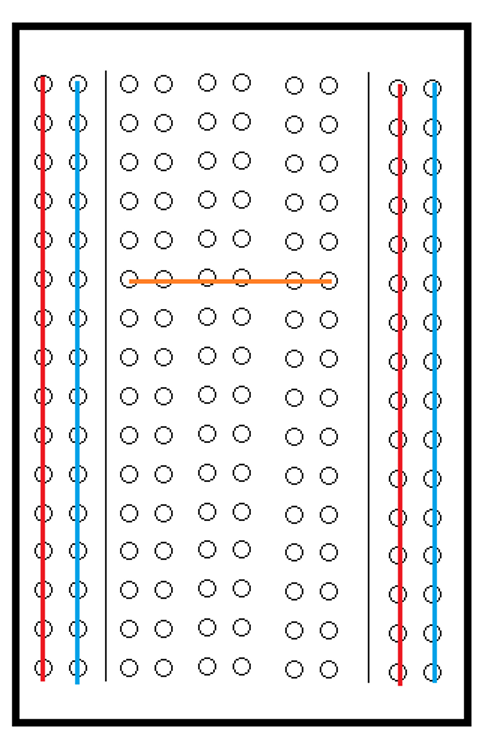
\includegraphics[width=0.25\linewidth]{figures/bread.png}
    \caption{麵包板線路排列示意圖}
    \label{fig:bread}
\end{figure}
\newline
    麵包板上方的孔以此連接方式有以下好處:
    \begin{itemize}
        \item 元件腳位可直接插入孔位,不需焊接即可達成電路串聯或並聯
        \item 電源和接地可直接藉由上方橫排分佈,方便供給各縱排相同的跨壓
    \end{itemize}

\subsection{示波器與三用電表的差別}\label{subsec:2}
% \hfill

\begin{itemize}
    \item 示波器:\\
    為一種時域(Time Domain)測量儀器,其作用是將電壓訊號轉換為可視化的波形,並顯示在螢幕上。可透過示波器觀察訊號的形狀、振幅、頻率和相位,及直流偏移等等。
    \newline
    主要經由四個步驟:
    \begin{enumerate}
        \item 訊號輸入:電訊號經由探棒進入示波器輸入端
        \item 模數轉換:訊號進入垂直放大器調整其適當的電壓範圍,再進入類比數位轉換器,將電壓訊號轉成數位訊號
        \item 時基與掃描:依照所設之取樣率擷取訊號數據點,並重建波形
        \item 顯示即及處理:透過處理單元將電壓對應到時間,繪出及時波形;並顯示時螢幕上(X軸表示時間、Y軸表示電壓)
    \end{enumerate}
    \clearpage
    \item 三用電表:\\
    一種測量電壓、電流、電阻的測量儀器。
    \newline
    主要可測數值之原理如下:
    \begin{enumerate}
        \item 直流電壓測量(DCV):採用電阻分壓分路來測量兩點間的電壓。公式如下:
        \begin{equation}
            V_{out} = V_{in} \frac{R_{2}}{R_{1}+R_{2}}
        \end{equation}
        其中$R_{1}$、$R_{2}$為內部電阻網路的分壓電阻。
        \item 交流電壓測量(ACV):利用整流電路和RMS轉換電路來測量交流訊號之有效值(即為上述提及之RMS);並透過整流二極體將AC轉為DC。
        \item 電流量測(A):串聯於電路中,利用分流電阻產生壓降,測量此壓降計算電流大小。電壓降根據歐姆定律為
        \begin{equation}
            V = IR
        \end{equation}
        \item 電阻測量($\Omega$):三用電表內部提供一已知電壓源,通過被測電阻產生電流,並根據歐姆定律計算電阻值。
    \end{enumerate}
    \item 兩者差異:
    \begin{center}
        \begin{tabular}{c|c|c}
         特性 &   示波器 &   三用電表  \\
         \hline
         \hline
         主要功能   &   顯示訊號波形   & 測量電壓(V)、\\
            &   分析時域特性  &   電流(A)、電阻($\Omega$)\\
        \hline
        測量方式    &   顯示隨時間變化的波形  &   顯示單一數值\\
        \hline
        測量結果    &   波形圖形化顯示 &   數值顯示\\
            &   可分析頻率、振幅、相位等等   &   有效值或平均值\\
        \hline
        交流訊號    &   可顯示瞬時值和波形形狀 &   顯示有效值(RMS)\\
        \hline
    \end{tabular}
    \end{center}
    
\end{itemize}

\subsection{解釋程序三所得的結果。哪種電錶可量到較高頻的交流信號? 在低頻(100Hz)時,$V_{pp}$ 和 ACV 檔的讀值有何關係?}\label{subsec:3}
\hfill

當量測訊號為正弦波,在低頻範圍(100Hz)使用電表測得的是RMS(均方根)電壓。正弦波的RMS值可以用公式計算:
\begin{equation}
    V_{rms} = \sqrt{\frac{1}{T}\int^{T}_{0}v^{2}(t)dt}        
\end{equation}
理論上測得的$V_{pp}$與 ACV 會符合 RMS 計算公式。\\
對於正弦波,$V_{pp}$與 ACV的關係為:
\begin{equation}
    V_{rms} = \frac{V_{pp}}{\sqrt{2}}
\end{equation}
量測低頻訊號(100Hz)時,ACV檔位的量測數值因電表的特性而產生偏差,導致ACV實際讀值小於理論值。同時DC offset影響ACV讀值,表示電表的AC測量可能缺乏高通濾波,也就是AC耦合。

若要量測到更精確的高頻交流訊號,應使用具高頻響應與具備一定RMS量測精確度的量測工具,如 True RMS 萬用電錶。

DC offset 除了會讓訊號在波形上產生偏移,在使用某些無法正確分辨出AC與DC訊號的量測工具(如三用電表)時,會導致量測出的數據與理論數字有落差。三用電表的ACV量測內建低通濾波器,頻率約為50Hz ~ 1kHz ,故在參數頻率為100kHz時,AC訊號已超出量測範圍 。且三用電表的 ACV 測量在接近其上限頻率時可能開始衰減,而非直接完全無法測量,故讀值顯示為 $<$0.00V。

量測低頻訊號(100Hz)時, ACV 讀值應為純 AC 訊號的 RMS 值 ,但ACV檔位的量測數值可能因電表的頻率響應而產生偏差,導致ACV實際讀值小於理論值。理論上 ACV 讀值不應受 DC Offset 影響,但由於三用電表缺乏高通濾波(AC 耦合功能),導致DC offset也會影響ACV讀值。相較之下,DCV 只取 DC Offset,不受頻率影響,應該等於設定的 Offset 值。

三用電表因為在高頻時可能會導致AC讀值衰減。若選用示波器進行量測,則可得出更精準的RMS值。

\subsection{由程序四的結果,我們可以用一個簡單模型來模擬電錶在歐姆檔的情形;請畫一個表,列出電錶不同檔之$V_{a}$與$R_{out}$}\label{subsec:4}
\hfill

\begin{center}
        \begin{tabular}{c|c|c}
        $\Omega$檔位  &  內部電壓$V_{a}$(V)   &   內部等效電阻
        $R_{out}$($\Omega$)\\
        \hline
        \hline
        20M &   \textcolor{red}{0.22}    &   \textcolor{red}{$\gg$1M}\\\hline
        200k    &   \textcolor{red}{0.41}    &   \textcolor{red}{few hundreds k}\\\hline
        20k    &   \textcolor{red}{0.41}    &   \textcolor{red}{$\sim$365}\\\hline
        2k    &   \textcolor{red}{0.42}    &   \textcolor{red}{$\sim$4}\\\hline
        200    &   \textcolor{red}{0.40}    &   \textcolor{red}{few}\\\hline
        \end{tabular}
    \end{center}
    總結上述,可看出:
    \begin{enumerate}
        \item 較高阻檔(20M$\Omega$、200k$\Omega$):內部阻抗極高,適合測量高組值電阻
        \item 中等阻檔(20k$\Omega$):內部阻抗約 365$\Omega$,適合測量 k$\Omega$ 級電阻
        \item 較低阻檔 (2k$\Omega$、200$\Omega$):內部阻抗較低,影響測量結果,適合測小電阻,但誤差較大
    \end{enumerate}

\subsection{由程序五步驟1的結果,求出電錶 DCV 檔之輸入阻抗}\label{subsec:5}
\hfill

當三用電錶測量時,會形成一個串聯電路,包含電源、負載電阻$R_{L}$和三用電錶內部阻抗$Z_{m}$;直流電壓輸出為$V_{in}$,測得電壓$V_{out}$會因為內部阻抗造成電壓下降,公式如下:
\begin{equation}
    V_{out} = V_{in} \frac{R_{L}}{R_{L}+Z_{m}}
\end{equation}
將每組數據帶入,可得出$Z_{m}$約為9.75k$\Omega$




\end{CJK}
\end{document}
